\documentclass{article}
\usepackage[margin=2cm]{geometry}
\usepackage{tikz}
\usetikzlibrary{arrows.meta}
\begin{document}

\title{Homework \#2}
\author{ECGR 5100, Fall 2022 \\
        Vishakha Dixit \\
        (801265288) \\
\texttt{vdixit2@uncc.edu}}
\date{November 08, 2022}
\maketitle

\begin{enumerate}
\item   Let $A$ be the set of the letters in the word ``trivial''
        \[ A = \{a,i,l,r,t,v\} \]
        and let $B$ be the letters in the word ``difficult.''
        \begin{enumerate}
        \item   Find $A \cup B$
        \item   Find $A-B$
        \item   What would the universe of discourse, $\cal U$, be?
        \item   Given $\cal U$, find $(A' \cup B')$
        \end{enumerate}

        \textbf{\underline {Soln-1}} Given: A = \{t, r, i, v, a, l\} and B = \{d, i, f, c, u, l, t\}
        \begin{enumerate}
            \item $A \cup B$ = \{a, c, d, f, i, l, r, t, u, v\}
            \item $A-B$ = \{r, v, a\}
            \item A Universe U is the larger set which gives the context. For our case we can consider U as a universal set of all possible letters in English alphabet.
            \item For given Universe U, $(A' \cup B')$ will contain all the elements that are neither in set A nor in set B as shown below: \\
            $(A' \cup B')$ = \{b, e, g, h, j, k, m, n, o, p, q, s, w, x, y, z\}           
        \end{enumerate}

\item   A survey of households in the United States reveals that
        96\% have at least one screen (TV set, computer monitor,
        projector), 98\% have cable service, and 95\% have cable
        service and at least one screen.  What, if anything, can
        you say about the households that have neither cable service
        nor a screen?  Explain your reasoning in a short paragraph
        ($2-5$ sentences).

        \textbf{\underline{Soln-2}} Given:
        \begin{itemize}
        \item {A - } At least one screen = 96\% 
        \item {B - } have cable service = 98\% 
        \item $A \cap B$: At least one screen and have cable service = 95\% 
        \\ A intersection B means households have at least one television set and have cable service which is 95\% we need to calculate 
        households which have neither television set nor internet service which is $\neg(A \cup B)$.
        \\ We know $A \cup B$ = $A + B - (A \cap B)$ 
        \\ Therefore, 
        \item $A \cup B$ = $0.96 + 0.98 - 0.95$ 
        \item $A \cup B$ = $0.99$ 
        \\ So, $\neg (A \cup B)$ will be $(1 - 0.99)$ which is 0.01 = 1\% of households have neither screen nor cable service.
        \end{itemize}

\item   Given the relation that you discovered in the process of doing
        a research project
        \[ R = \left\{ \langle x, x^2 \rangle \middle|
                -\infty < x < \infty \right\} \]
        \begin{enumerate}
        \item   Is $R$ a function?
        \item   Is $R$ an injection?  If not, give an example.
        \item   Is $R$ a surjection?  If not, give an example.
        \end{enumerate}
        How would you go about proving your answers above?  Have
        you introduced any assumptions that might change your answers?
        (For example, if $R \subseteq S \times T$, what are $S$ and $T$?)
        \par
        \emph{\textbf{Now}}, assuming you understand $R$ well now,
        write a paragraph
        ($3-5$ sentences) for the average reader with a college (B.S.)
        degree, what you can say about $R$ and what you prove about whether
        or not $R$ is a bijection.

        \textbf{\underline{Soln-3}} 
        \begin{enumerate}
            \item   For a given Relation R, we can say that R is a Function because every element x in set S has a unique mapping to every element of $x^2$ in set T.
            \item   Given Relation R is not Injection. \\
            For example, \\
            If we have set S = \{-3, -2, 3, 4\} then set T = \{9, 16\} \\
            then R = $\left\{ \langle x, x^2 \rangle \middle|-\infty < x < \infty \right\}$ = \{(-3,9), (-2, 4), (3, 9), (4, 16)\}. \\
            Therefore, we can see that -3 and 3 in set S are mapped to same element 9 in set T, 
            which contradicts the definition of Injection function as Injective function is a function where no two elements from set S 
            should be mapped to same element in set T.
            \item  Given Relation R is Surjective. \\
            For example: \\
            If we have set S = \{-3, -2, 3, 4\} then set T = \{9, 16\} \\
            then R = $\left\{ \langle x, x^2 \rangle \middle|-\infty < x < \infty \right\}$ = \{(-3,9), (-2, 4), (3, 9), (4, 16)\}. \\
            We can see that every element $x^2$ in set T has mapping to every element in set S. Therefore, R is Surjective.
        \end{enumerate}

        The Given Relation R is not Bijection because for a function to be Bijective it must be both Injective and Surjective. 
        Whereas in our case the given relation is not Injective, therefore we can say that R is not Bijective.

\item   Let $V$ be the set of vowels in English
            \[ V = \{a,e,i,o,u,y\} \]
        and the relation $R$ be ``$u$ comes before $v$ in the usual
        alphabetic order or if $u=v$'' where $u,v \in V$.
        \begin{enumerate}
        \item   Is $V$ the universe of discourse?  Is $R$ reflexive?
        \item   Is $R$ antisymmetric?  Would your answer change if
                ${\cal U}$ was alphabet $a$, $b,$ ... $z$?
        \item   Is $R$ transitive?  If not, can you prove it?
        \end{enumerate}
        \par
        \emph{Given your understanding of this relation}, write a paragraph
        the proves or disproves that $R$ is partial order.

        \textbf{\underline{Soln-4}} Given: V = \{a, e, i, o, u\} and relation R = “u comes before v in the usual alphabetic order or 
        if u = v” where $(u, v) \epsilon V$. \\
        With the given definition above we get: \\
        R = \{(a, e), (a, i), (a, o), (a, u), (e, i), (e, o), (e, u), (i, o), (i, u), (o, u), (a, a), (e, e), (i, i), (o, o), (u, u)\}
        
        \begin{enumerate}
            \item Given set V is not the Universe of Discourse. \underline{R is a reflexive} because R can contain pairs \(u, v\) such that u = v.
            \item \underline{R is antisymmetric} because R can contain all pairs of \(u, v\) and \(v, u\) such that u = v. If Universe of Discourse U contains 
                all alphabets from a to z, the relation R will still be antisymmetric as based on the definition of R it will still contain all the pairs 
                of \(u, v\) where u = v. Therefore, our answer will not change.
            \item Given relation \underline{R is transitive} because for every pair \(u, v\) and \(v, w\) there exists a pair \(u, w\) in the relation R.
        \end{enumerate}

        From the above solutions we can see that R is Reflexive, Antisymmetric, and Transitive. And for a relation to be partial order it must satisfy 
        these three characteristics. Therefore, we can say that R is partial order relation.

\item   Given the following scenario, build up a formal
        mathematical description of the system.
        \begin{quote}
            A discrete mathematics course contains 1 mathematics
            major who is a freshman, 12 mathematics majors who are
            sophomores, 15 computer engineering majors who are sophomores,
            and 2 mathematics majors who are juniors, 2 computer
            engineering majors who are juniors,
            and 1 computer engineering major who is a senior.
        \end{quote}
        Express each of these statements as quantified predicates
        and \emph{prove} its truth value.
        \begin{enumerate}
        \item   There is a student in the class who is a junior.
        \item   Every student in the class is a computer engineer.
        \item   There is a student in the class that is neither
                a sophomore nor a junior.
        \item   There is a student in the class that is neither
                a sophomore nor a junior.
        \item   There is a major such that there is a student in
                the class in every year of study with that
                major.
        \end{enumerate}

        \textbf{\underline{Soln-5}} Let’s consider predicate P(s, c, m) as statement that Student \textbf{s} who has standing Class \textbf{c} and is Majoring in \textbf{m}. 

        \begin{enumerate}
            \item The preposition is $\exists s \exists mP(s, junior, m)$. It is true for given information.
            \item The preposition is $\forall s \exists cP(s, c, computer engineering)$. This is false, because there are some students who have mathematics major.
            \item The preposition is $\exists s \exists c \exists m(P(s, c, m) \wedge c \neq sophmore \wedge c \neq junior)$. This is a true, as there is a freshman majoring in mathematics.
            \item The preposition is $\exists m \exists s \forall y [InClass(s) \wedge Major(s,m) \wedge Year(s,y)]$. This is false, as there is no student in computer engineering who is Freshman.
        \end{enumerate}

\item   Given the following illustration of a graph $G$, answer these
        basic questions about $G$.
        \begin{center}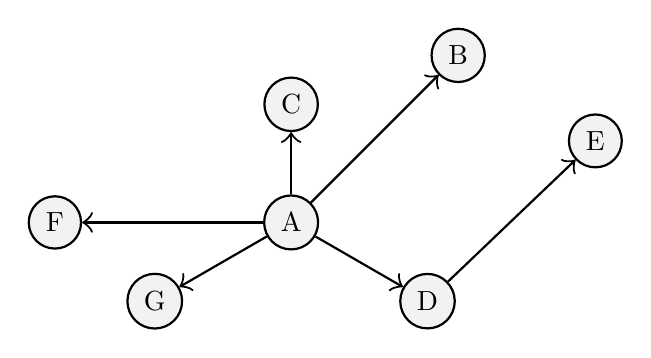
\begin{tikzpicture}[
          every node/.style={
            draw,
            thick,
            circle,
            fill=black!5,
            minimum size=10pt,
          },
          thick,
          foo/.tip={>[scale=2]},
          >={Classical TikZ Rightarrow[scale=1.5]},
        ]
        \node (root) {A} ;
        \node at (45:3) (b) {B} ;
        \node at (90:1.5) (c) {C} ;
        \node at (-30:2) (d) {D} ;
        \node at (15:4) (e) {E} ;
        \node at (180:3) (f) {F} ;
        \node at (210:2) (g) {G} ;
        \draw[->] (root)--(b) ;
        \draw[->] (root)--(c) ;
        \draw[->] (root)--(d) ;
        \draw[->] (d)--(e) ;
        \draw[->] (root)--(f) ;
        \draw[->] (root)--(g) ;
        \end{tikzpicture}\end{center}
        \begin{enumerate}
        \item   Define graph $G$ formally.
        \item   Is $G$ an undirected graph?
        \item   Is $G$ formally a tree?  If yes,
                \begin{itemize}
                \item   what is the root of $G$?
                \item   what is the height of $G$?
                \item   how many cycles are in $G$?
                \end{itemize}
        \end{enumerate}

        \textbf{\underline{Soln-6}} 
        \begin{enumerate}
            \item The given Graph can be formally defined as G = (V, E), where V stands for Vertices, and E stands Edges. \\
                V = \{A, B, C, D, E, F, G\} \\
                E = \{(A, B), (A, C), (A, D), (D, E), (A, F), (A, G)\}
            \item The given graph is not an undirected graph as the relationship between the Vertices are not symmetric. 
            \item G is formally a tree as it is acyclic, directed, and connected.
            \begin{itemize}
                \item The root of G is node A.
                \item The height of G is 2.
                \item There are no cycles in G.
            \end{itemize}
        \end{enumerate}

\item   Let $T$ be a binary tree that is constructed as follows.
        Given a node $n$ and a datum $x$, an \texttt{\textbf{add()}}
        operation will...
        \begin{itemize}
        \item   set $n$ to be a new node with $x$ as the datum
                and left=right=NULL
        \item   (recursively) add $x$ to sub-tree $n$.left
                if $x$ is greater-than-or-equal-to $n$'s datum
        \item   (recursively) add $x$ to sub-tree $n$.right
                if $x$ is less-than $n$'s datum
        \end{itemize}
        Draw (illustrate) the tree for the inputs:  5,7,4,3,4,5

        \textbf{\underline{Soln-7}}

        \begin{center}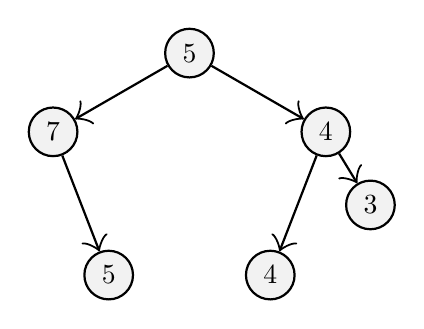
\begin{tikzpicture}[
            every node/.style={
              draw,
              thick,
              circle,
              fill=black!5,
              minimum size=10pt,
            },
            thick,
            foo/.tip={>[scale=2]},
            >={Classical TikZ Rightarrow[scale=2]},
          ]
          \node (root) {5} ;
          \node at (210:2) (b) {7} ;
          \node at (-30:2) (c) {4} ;
          \node at (250:3) (d) {5} ;
          \node at (-70:3) (e) {4} ;
          \node at (320:3) (f) {3} ;
          \draw[->] (root)--(b) ;
          \draw[->] (root)--(c) ;
          \draw[->] (b)--(d) ;
          \draw[->] (c)--(e) ;
          \draw[->] (c)--(f) ;
          \end{tikzpicture}\end{center}

\item   A binary tree $T$ visits nodes in the following order
        using an in-order traversal.
                \[ B-A-S-I-C \]
        \begin{enumerate}
        \item   Draw (illustrate) this tree graphically.
        \item   Is there more than one tree that will produce this
                output?
        \end{enumerate}

        \textbf{\underline{Soln-8}}
        \begin{enumerate}
            \item The binary tree for given in-order traversal can be represented as follows: 
            \begin{center}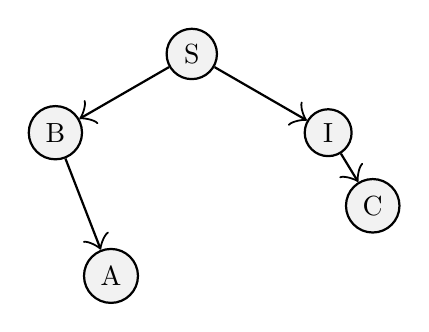
\begin{tikzpicture}[
                every node/.style={
                  draw,
                  thick,
                  circle,
                  fill=black!5,
                  minimum size=10pt,
                },
                thick,
                foo/.tip={>[scale=2]},
                >={Classical TikZ Rightarrow[scale=2]},
              ]
              \node (root) {S} ;
              \node at (210:2) (b) {B} ;
              \node at (-30:2) (c) {I} ;
              \node at (250:3) (d) {A} ;
              \node at (320:3) (f) {C} ;
              \draw[->] (root)--(b) ;
              \draw[->] (root)--(c) ;
              \draw[->] (b)--(d) ;
              \draw[->] (c)--(f) ;
              \end{tikzpicture}\end{center}

              \item Yes, two structureally different trees can have same inorder traversal output. For example, tree shown below produces same output as above on inorder traversal.
              \begin{center}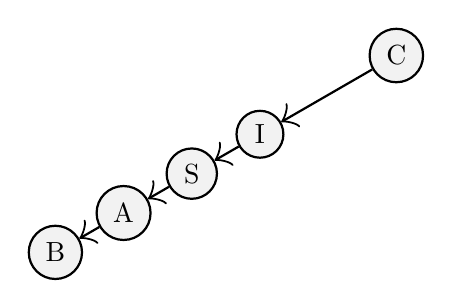
\begin{tikzpicture}[
                every node/.style={
                  draw,
                  thick,
                  circle,
                  fill=black!5,
                  minimum size=10pt,
                },
                thick,
                foo/.tip={>[scale=2]},
                >={Classical TikZ Rightarrow[scale=2]},
              ]
              \node (root) {C} ;
              \node at (210:2) (b) {I} ;
              \node at (210:3) (c) {S} ;
              \node at (210:4) (d) {A} ;
              \node at (210:5) (f) {B} ;
              \draw[->] (root)--(b) ;
              \draw[->] (b)--(c) ;
              \draw[->] (c)--(d) ;
              \draw[->] (d)--(f) ;
              \end{tikzpicture}\end{center}
        \end{enumerate}


\end{enumerate}
\end{document}
